\section{Comandos de \LaTeX}
Algunos de los principales comandos son:
\begin{table}[H]
    \centering
    \begin{tabular}{l l}
        \symbol{92}textit   & Permite escribir en \textit{itálica}. \\
        \symbol{92}textbf   & Permite poner en \textbf{negrilla} un texto. \\
        \symbol{92}sout     & Nos permite \sout{tachar} texto. \\
        \symbol{92}texttt   & Permite escribir texto con una \texttt{fuente monoespaciada}. \\
        \symbol{92}footnote & Permite agregar pies de página y una referencia a ella. \\
        \symbol{92}newpage  & Permite hacer un salto de página.\\
        \symbol{92}nameref{referencia} & Permite hacer referencias en el contenido\\
        \%     & Permite comentar todo texto que se encuentre a la derecha de este símbolo.
    \end{tabular}
\end{table}

%%%%%%%%%%%%%%%%%%%%%%%%%%%%%%%%%%%%%%%%%%%%%%%%%%%%%%%
\section{Organización}

\subsection{Secciones}
Pueden organizar el documento en distintas secciones y sub-secciones, lo que nos permite tener todo más ordenado, facilitando así la lectura. Actualmente, existen los siguientes niveles de organización:

\begin{table}[H]
    \centering
    \begin{tabular}{l l}
        \symbol{92}section\{\}       & \Large{\textbf{1.\hspace{.5cm} Secciones}} \\
        \symbol{92}subsection\{\}    & \large{\textbf{1.1.\hspace{.3cm} Subsecciones}} \\
        \symbol{92}subsubsection\{\} & \textbf{1.1.1.\hspace{.05cm} Subsubsecciones} \\
    \end{tabular}
\end{table}

\subsection{Listados}
Hay diferentes formas de listar elementos\footnote{Pueden usarse varias cosas, más info en el siguiente \href{https://es.overleaf.com/learn/latex/Lists}{link}}
\begin{multicols}{3}
    Uso de \texttt{itemize}
    \begin{itemize}
        \centering
        \item Elemento
        \item Elemento
        \item Elemento
    \end{itemize}
    
    \columnbreak % Para separar columna
    
    Uso de \texttt{enumerate}
    \begin{enumerate}
        \centering
        \item Elemento
        \item Elemento
        \item Elemento
    \end{enumerate}
    
    \columnbreak% Para separar columna x2
    
    Uso de elemento personalizado
    \begin{itemize}[$\blacksquare$] % o *, +, o, etc
        \centering
        \item Descripción
        \item Descripción
        \item Descripción
    \end{itemize}
\end{multicols}


%%%%%%%%%%%%%%%%%%%%%%%%%%%%%%%%%%%%%%%%%%%%%%%%%%%%%%%
\newpage
\section{Imágenes}
\subsection{Imagen centrada}
En esta plantilla hay 2 formas de incluir imágenes. La primera es la más compleja y manual que aparece en el código comentado.
%\begin{figure}[H] % IMPORTANTE en la mayoria de los casos, alternativas: [h],[t],[b],[p],
%    \centering
%    \begin{measuredfigure} % Lo usamos para aliniar el caption
%        \caption{Título de la imagen} % IMPORTANTE que este arriba
%        
\includegraphics[width=0.2\textwidth]{img/cuadradoejemplo.png} % Alternativa \includegraphics[height=3cm]{}
%        \label{img:referencia0}
%    \end{measuredfigure}
%\end{figure}

La segunda forma de incluir imágenes es la más sencilla, solo se tiene que usar el comando personalizado:
\begin{verbatim} 
\fig[label]{Titulo}{tamaño}{ruta_imagen}
\end{verbatim}

\fig[referencia1]{Titulo de la imagen 1}{width = 0.2\textwidth}{img/cuadradoejemplo.png}

% Tambien se puede agregar sin caption ni label ni titulo:
% \fig{}{width = 0.2\textwidth}{img/cuadradoejemplo.png}

\subsection{Imágenes alineadas}
Sin embargo, si se desea incluir una imagen a la izquierda o derecha de un párrafo, se puede hacer lo siguiente (Poniendo \{r\} o \{l\} dependiendo del caso):

\begin{wrapfigure}{r}{0.2\textwidth} % Margen del texto
    \centering
    \begin{measuredfigure}
        \caption{Imagen referencia 2}
        
\includegraphics[height=3cm]{img/cuadradoejemplo.png} %[scale=0.1]
        \label{img:referencia2}
    \end{measuredfigure}
\end{wrapfigure}


\textcolor{silver}{
    Ahora generaremos algo de texto aleatorio:
    \lipsum[2]
}

\subsection{Imágenes que rompen márgenes}

Este es un caso muy particular, en el que se quiera incluir una imagen decorativa en algún estilo. En este caso de ejemplo, incluiremos una imagen en la base ([b]) al "south east", aunque también se puede incluir en "west" y personalizar de otras maneras.

\begin{figure}[b]
    \begin{tikzpicture}[remember picture, overlay]
    \node[anchor=south east, % west
        xshift=0mm,
        yshift=0mm,
        opacity=1]
        at (current page.south east)  % west
        {
\includegraphics[height=3cm]{img/cuadradoejemplo.png}}; 
        %(box) at (-2cm,0)(box){\includegraphics[scale=1]{img/circulos-amarillo3.png}};
    \end{tikzpicture}
    %\caption{Ilustración}
    %\label{fig:Ilustración}
\end{figure}

\newpage

%%%%%%%%%%%%%%%%%%%%%%%%%%%%%%%%%%%%%%%%%%%%%%%%%%%%%%%
\section{Tablas}

Hacer tablas en \LaTeX es muy engorroso, por lo que presentamos 3 alternativas. Sin embargo, es necesario aclarar que para que se respete el formato de las tablas, \textbf{se tiene que poner el catión SOBRE la tabla.}

\subsection{Generador online}
Hay muchas páginas para generar tablas automáticamente, una alternativa es \href{tablesgenerator}{https://www.tablesgenerator.com}, sin embargo, este método genera muchas líneas innecesarias y cuando se incorporan párrafos muy grandes hay que ajustar las palabras.

\subsection{Insertar una imagen como tabla}
Se puede incorporar una imagen (De Excel, por ejemplo) como si fuera una tabla. El único inconveniente es que no va a permitir seleccionar el texto en el pdf generado.
\begin{table}[H]
    \centering
    \caption{Tabla de referencia 1}
    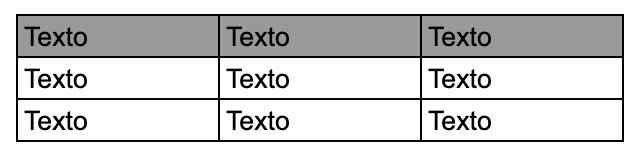
\includegraphics[height=3cm]{img/tablaejemplo.png} 
    \\ \textit{\scriptsize{Texto opcional al el pie de Tabla.}}
    \label{img:referencia3}
\end{table}


\subsection{Usar plantilas}
\begin{minipage}[H]{0.49\textwidth}
    \begin{table}[H]
        \centering
        \caption{Tabla de referencia 2}
        \begin{tabular}{| l | c | r |} 
        \hline
            \textbf{Texto} & \textbf{Texto} & \textbf{Texto} \\ \hline
            Textoblabla    & Textoblabla   & Textoblabla \\ \hline
            Texto    & Texto   & Texto \\ \hline
        \end{tabular}
        \\ \textit{\scriptsize{Texto opcional al el pie de Tabla.}}
    \end{table}
\end{minipage}
\begin{minipage}[H]{0.49\textwidth}
    \begin{table}[H]
        \centering
        \caption{Tabla de referencia 3}
        \begin{tabular}{l l l}
        \toprule
            \textbf{Texto} & \textbf{Texto} & \textbf{Texto} \\
            \midrule
            Textoblabla    & Textoblabla   & Textoblabla \\
            Texto    & Texto   & Texto \\
            \bottomrule
        \end{tabular}
        \\ \textit{\scriptsize{Texto opcional al el pie de Tabla.}}
    \end{table}
\end{minipage}

%%%%%%%%%%%%%%%%%%%%%%%%%%%%%%%%%%%%%%%%%%%%%%%%%%%%%%%
\newpage
\section{Código}
\subsection{pseudocódigo}
Para generar un pseudo código en blanco y negro se pueden basar en el siguiente estilo (Es importante la tabulación):

\texttt{PSEUDOCODIGO(A)} % Lo recomiendo defar fuera
\begin{lstlisting}[style=blancoynegro]
    i = 3
    while A <= i do
        print uwu
        i --
    end while
\end{lstlisting}

\subsection{Python}
Para escribir código como si fuera Python, se pueden basar en el siguiente estilo:
\begin{lstlisting}[language=Python, style=stylepython]
    def funcionpython(A):
        i = 3
        while True:
            print("UwU") # OwO
\end{lstlisting}

\subsection{json}
\begin{minted}[linenos,frame=single]{json} 
[
  {
    "palabra": "texto",
    "palabra": "texto",
    "id": 0
  }
]
\end{minted}

\subsection{Alternativa}
Sí usamos \symbol{92}begin\{verbatim\} podemos organizar con comodidad.
\begin{verbatim}
    1
    HOLA 4
    20 3
    FIN
\end{verbatim}

% Si se quiere poner \ se puede usar \symbol{92}

%%%%%%%%%%%%%%%%%%%%%%%%%%%%%%%%%%%%%%%%%%%%%%%%%%%%%%%
\newpage
\section{Cajas de texto}
Usando \texttt{tcolorbox} se pueden hacer diferentes cajas para incluir ejemplos, teoremas y demás. Acá adjunto algunos ejemplos de internet.

\begin{tcolorbox}
  Mi caja.
\end{tcolorbox}

\begin{tcolorbox}[colback=red!5!white,colframe=red!75!black]
  Mi caja x2.
\end{tcolorbox}

\begin{tcolorbox}[colback=blue!5!white,colframe=blue!75!black,title=Mi titulo]
  Mi caja con titulo
\end{tcolorbox}

\begin{tcolorbox}[colback=green!5!white,colframe=green!75!black]
  Parte superior
  \tcblower
  Parte inferior
\end{tcolorbox}

\begin{tcolorbox}[colback=yellow!5!white,colframe=yellow!50!black,colbacktitle=yellow!75!black,sidebyside,title=Mi titulo]
  Parte izquierda (agregada con "sidebyside")
  \tcblower
  Parte derecha
\end{tcolorbox}

\begin{tcolorbox}[colback=yellow!10!white,colframe=red!75!black,lowerbox=invisible,
  savelowerto=\jobname_ex.tex]
  Parte superior
  \tcblower
  Soy un texto invisible
\end{tcolorbox}

\begin{tcolorbox}[colback=yellow!10!white,colframe=red!75!black,title=Aparece el titulo invisible]
  \input{\jobname_ex.tex}
\end{tcolorbox}


%----------------------------------------------------------
\begin{tcolorbox}[enhanced,watermark graphics=img/cuadradoejemplo.png, watermark opacity=0.3,watermark zoom=0.9, colback=green!5!white,colframe=green!75!black, fonttitle=\bfseries, title=Titulo]
      Soy un texto creado solo para rellenar esta caja y mostrar que en el fondo hay una imagen como mascara y oculta con un degrade.
\end{tcolorbox}

%----------------------------------------------------------
\begin{tcolorbox}[colback=yellow!10!white,colframe=yellow!50!black,every box/.style={fonttitle=\bfseries},title=Caja1]
  \begin{tcolorbox}[enhanced,colback=red!10!white,colframe=red!50!black,colbacktitle=red!85!black,title=Caja2]
    \begin{tcolorbox}[beamer,colframe=blue!50!black,title=Caja3]
      Soy un texto de ejemplo!\par\medskip
      \newtcbox{\mybox}[1][]{nobeforeafter,tcbox raise base,colframe=green!50!black,colback=green!10!white,sharp corners,top=1pt,bottom=1pt,before upper=\strut,#1}
      \mybox[rounded corners=west]{Esta}
      \mybox{es}
      \mybox{una}
      \mybox[rounded corners=east]{caja!}
    \end{tcolorbox}
  \end{tcolorbox}
\end{tcolorbox}


